\section{Custom Layout Design Functions in Software}
\label{sec:parameterized}

OpenRAM provides classes that can be used to generated parameterized
cells for the most common cells: transistors, inverters, nand2, nand3, etc...  
There are many advantages to having parameterized cells.
The main advantage is that it makes it easier to dynamically generate designs and cuts
down the necessary code to be written.  
We also need parameterized cells because some designs, such as the wordline drivers, need to be
dynamically sized based on the size of the memory. 
Lastly, there may be certain physical dimension requirements that need to be met for a
cell, while still maintaing the expected operation/performance.  
In OpenRAM we currently provide five parameterized cells: parameterized
transistor (\verb|ptx|), parameterized inverter (\verb|pinv|), parameterized nand2 (\verb|nand_2|), 
parameterized nand3 (\verb|nand_3|) and parameterized nor2 (\verb|nor_2|). 


\subsection{Parameterized Transistor}
\label{sec:ptx}

The parameterized transistor class generates a transistor of specified
width and number of mults.
The \verb|ptx| is constructed as follows:
\begin{verbatim}
def __init__(self,name,width,mults,tx_type)
\end{verbatim} 

An explanation of the \verb|ptx| parameters is shown in
Table~\ref{table:ptx_params}. A layout of ptx, generated by the
following instatiation, is depicted in Figure~\ref{fig:ptx_example}.
\begin{verbatim}
fet = ptx.ptx(name = "nmos_1_finger", width = tech.drc["minwidth_tx"], 
mults = 1, tx_type = "nmos").
\end{verbatim}

\begin{table}[h!] 
  \begin{center}
    \begin{tabular}{| l | c |}
    \hline
    Parameter & Explanation  \\ \hline
    \verb|width| & active\_height \\ \hline
    \verb|mults| & mult number of the transistor \\ \hline
    \verb|tx_type| & type of transistor,”nmos” and “pmos” \\ \hline
    \hline
    \end{tabular}
  \end{center}
  \caption{Parameter Explanation of ptx}
  \label{table:ptx_params}
\end{table}


\begin{figure}[h!]
\centering
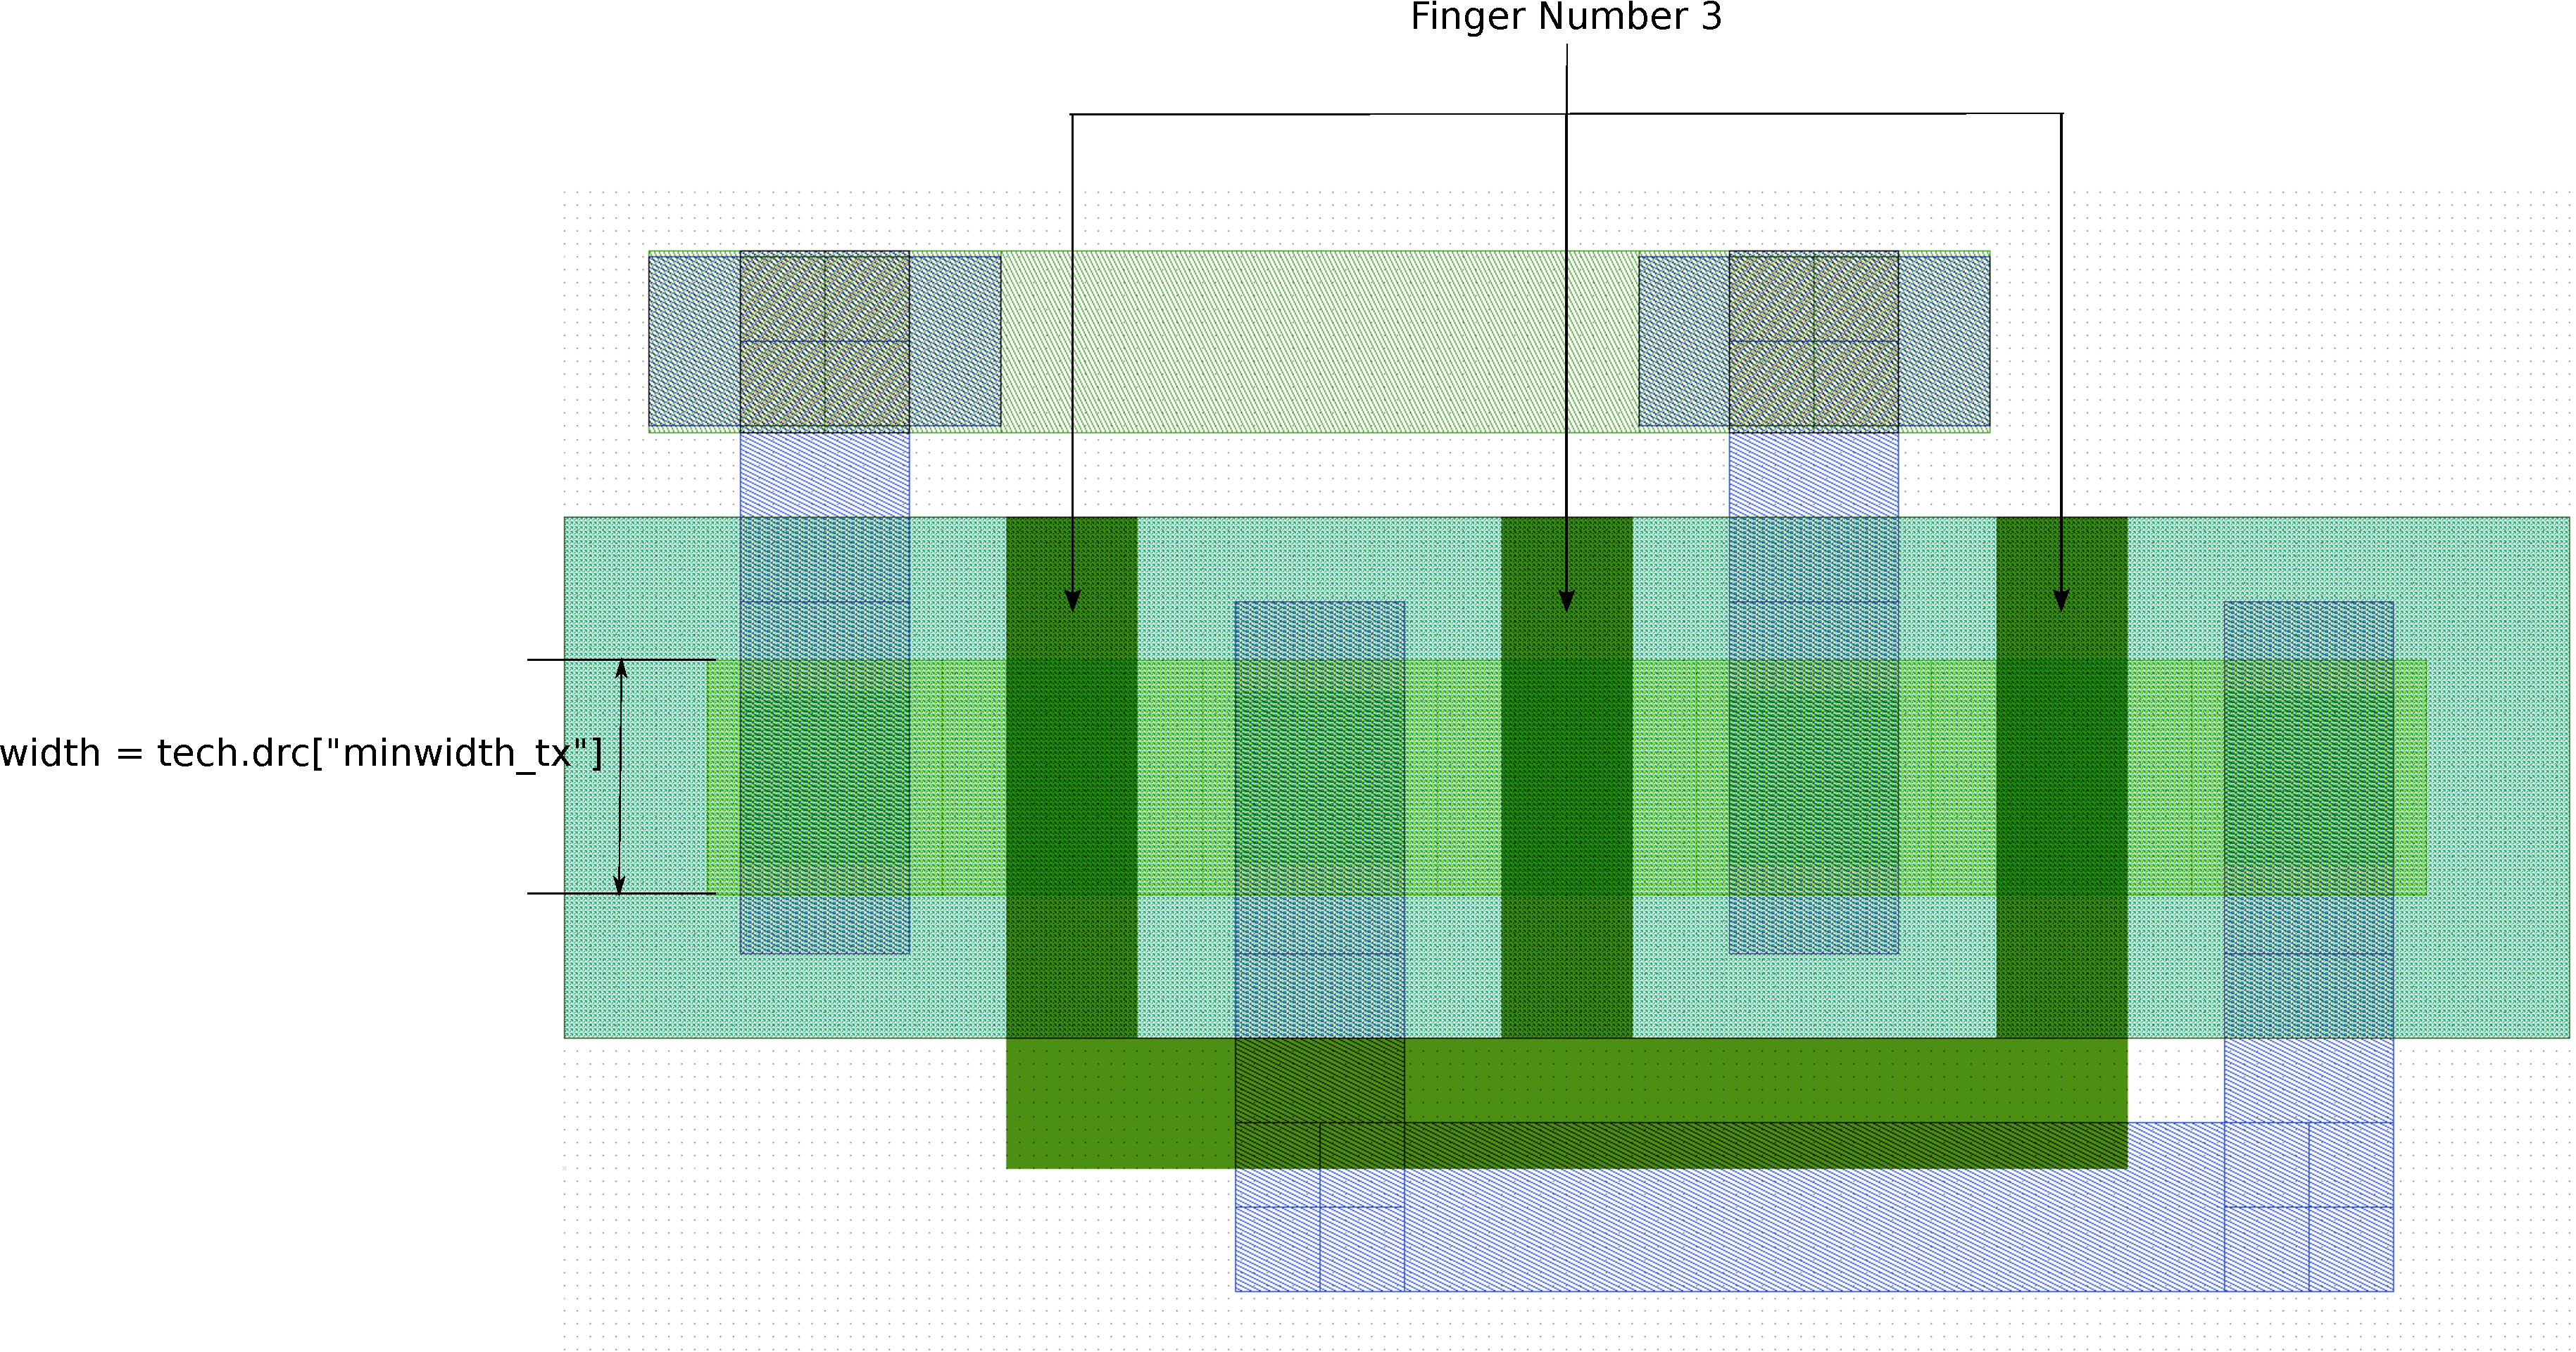
\includegraphics[width=10cm]{./figs/ptx.pdf}
\caption{An example of Parameterized Transistor (ptx)}
\label{fig:ptx_example}
\end{figure}



\subsection{Parameterized Inverter}
\label{sec:pinv}

The parameterized inverter (\verb|pinv|) class generated an inverter
of a specified size/strength and height.  The \verb|pinv| is
constructed as follows:
\begin{verbatim}
def __init__(self, cell_name, size, beta=tech.[pinv.beta], 
cell_size=tech.cell[height])
\end{verbatim}

The parameterized inverter can provide significant drive strength
while adhering to physical cell size limitations. That is achieved by
having many small transistors connected in parallel, thus the height
of the inverter cell can be manipulated without the affecting the
drive strength. The NMOS size is an input parameter, and the PMOS size
will be determined by $beta*NMOS\_size$, where beta is the ratio of
the PMOS channel width to the NMOS channel width.  The following code
instatiates the \verb|pinv| instance seen in Figure~\ref{fig:pinv}.
\begin{verbatim}
a=pinv.pinv(cell_name="pinv",size=tech.drc["minwidth_tx"]*8)
\end{verbatim}
\begin{figure}[h!]
\centering
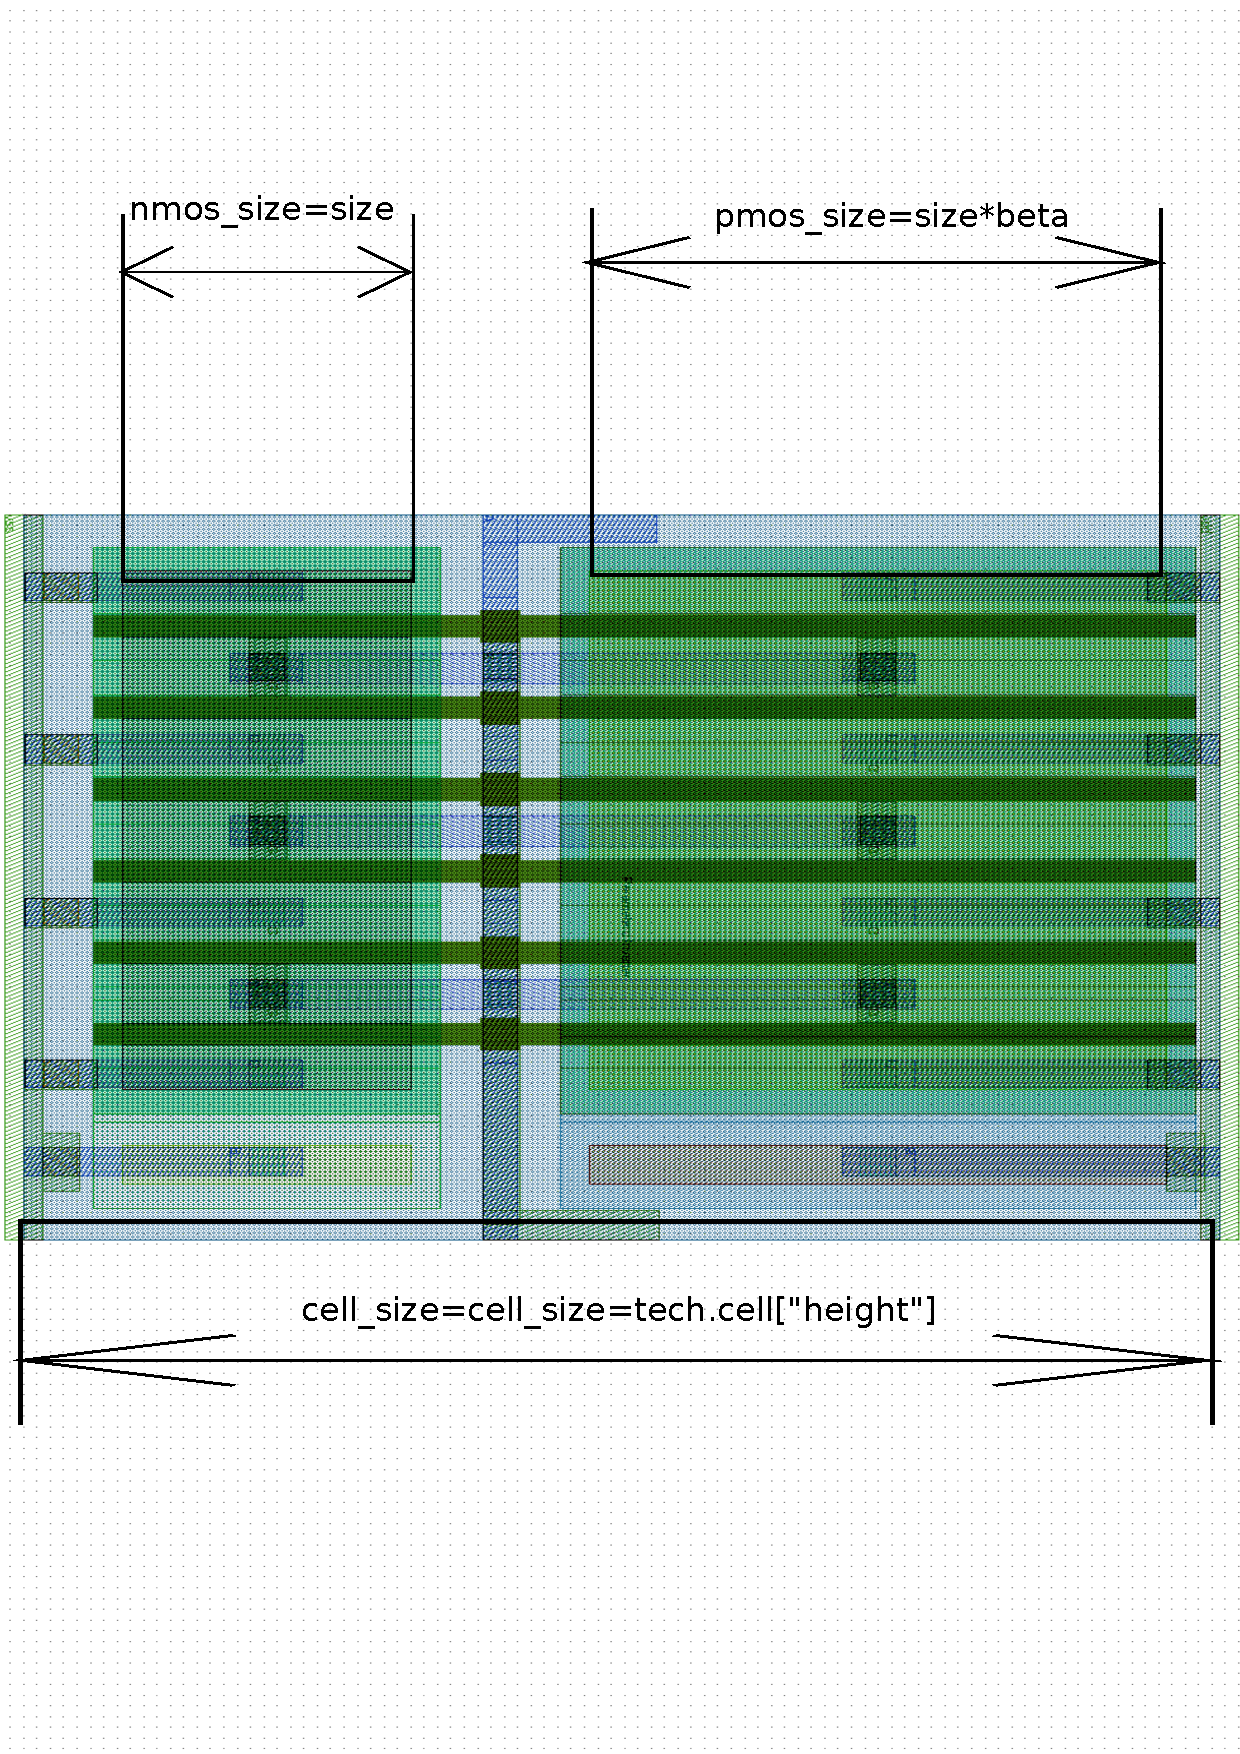
\includegraphics[width=10cm]{./figs/pinv.pdf}
\caption{An example of Parameterized Inverter(pinv)}
\label{fig:pinv}
\end{figure}


The \verb|pinv| parameters are explained in Table~\ref{table:pinv_params}.
\begin{table}[h!] 
  \begin{center}
    \begin{tabular}{| l | c |}
    \hline
    Parameter & Explanation \\ \hline
    \verb|size| & The logic size of the transistor of the nmos in the pinv \\ \hline
    \verb|beta| = tech.[pinv.beta] & Ratio of pmos channel width to nmos channel width. \\ \hline
    \verb|cell_size| = tech.cell[height] & physical dimension of cell height. \\ 
    \hline
    \end{tabular}
  \end{center}
  \caption{Parameter Explanation of pinv}
  \label{table:pinv_params}
\end{table}



\subsection{Parameterized NAND2}
\label{sec:nand2}

The parameterized nand2 (\verb|nand_2|) class generated a 2-input nand gate
of a specified size/strength and height.  The \verb|nand_2| is
constructed as follows:
\begin{verbatim}
def __init__(self, name, nmos_width, height=tech.cell_6t[height])
\end{verbatim}

The NMOS size is an input parameter, and the PMOS size
will be equal to NMOS to have the equal rising and falling for output. 
The following code instatiates the \verb|nand_2| instance seen in Figure~\ref{fig:nand2}.
\begin{verbatim}
a=nand_2.nand_2(name="nand2", nmos_width=2*tech.drc["minwidth_tx"], 
height=tech.cell_6t["height"])
\end{verbatim}

\begin{figure}[h!]
\centering
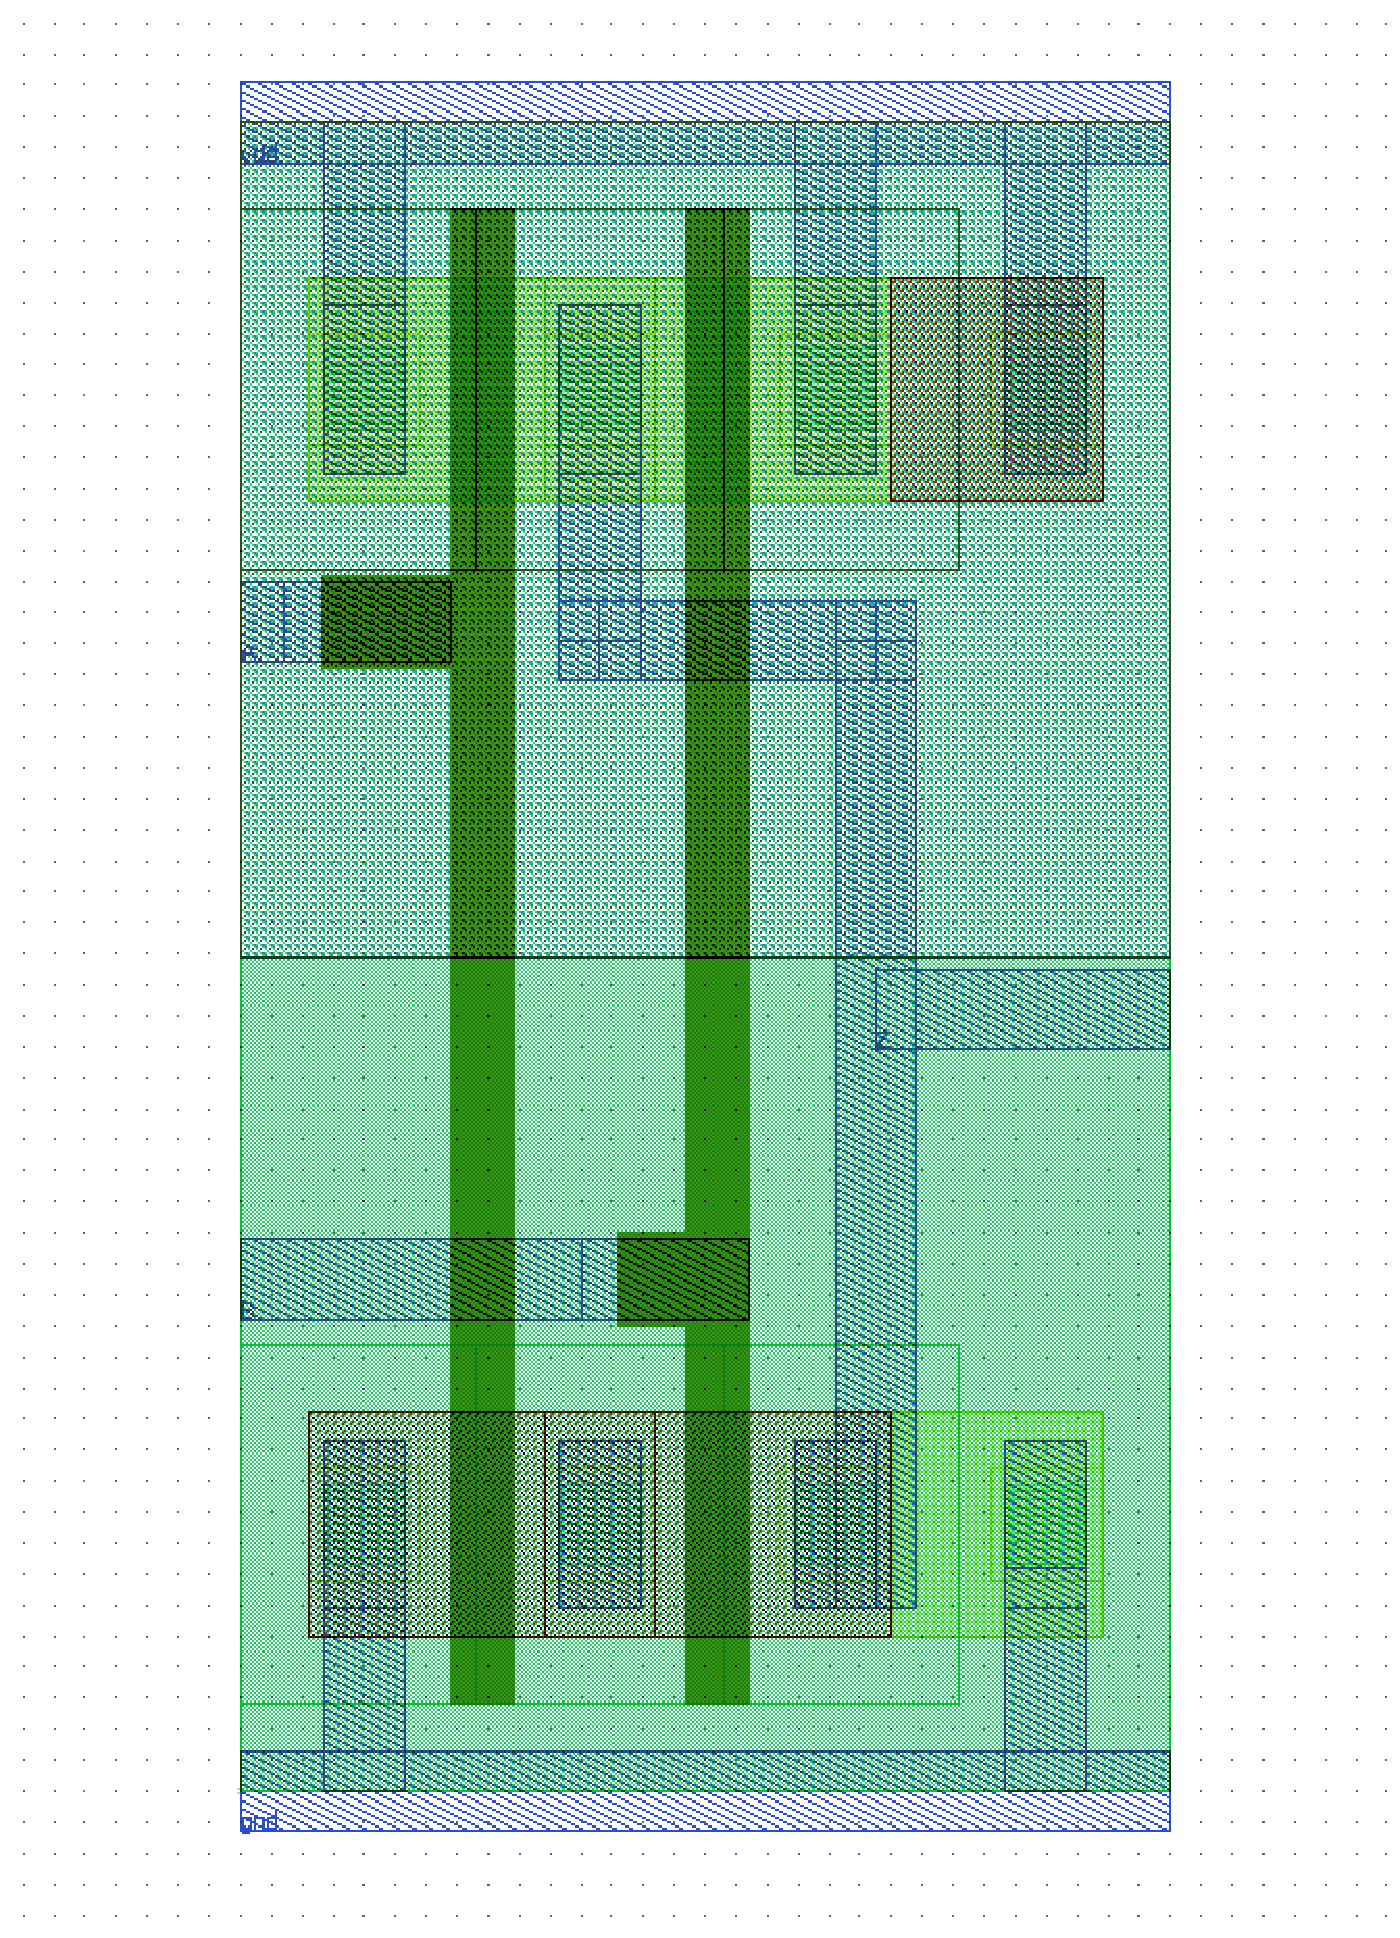
\includegraphics[width=10cm]{./figs/nand2.pdf}
\caption{An example of Parameterized NAND2(nand\_2)}
\label{fig:nand2}
\end{figure}


The \verb|nand_2| parameters are explained in Table~\ref{table:nand2_params}.
\begin{table}[h!] 
  \begin{center}
    \begin{tabular}{| l | c |}
    \hline
    Parameter & Explanation \\ \hline
    \verb|nmos_width| & The logic size of the transistor of the nmos in the nand2 \\ \hline
    \verb|height| = tech.cell\_6t[height] & physical dimension of cell height. \\ 
    \hline
    \end{tabular}
  \end{center}
  \caption{Parameter Explanation of nand2}
  \label{table:nand2_params}
\end{table}



\subsection{Parameterized NAND3}
\label{sec:nand3}

The parameterized nand3 (\verb|nand_3|) class generated a 3-input nand gate
of a specified size/strength and height.  The \verb|nand_3| is
constructed as follows:
\begin{verbatim}
def __init__(self, name, nmos_width, height=tech.cell_6t[height])
\end{verbatim}
The NMOS size is an input parameter, and the PMOS size
will be equal to $2/3$ NMOS size to have the equal rising and falling for output.
The following code instatiates the \verb|nand_3| instance seen in Figure~\ref{fig:nand3}.
\begin{verbatim}
a=nand_3.nand_3(name="nand3", nmos_width=3*tech.drc["minwidth_tx"], 
height=tech.cell_6t["height"])
\end{verbatim}


\begin{figure}[h!]
\centering
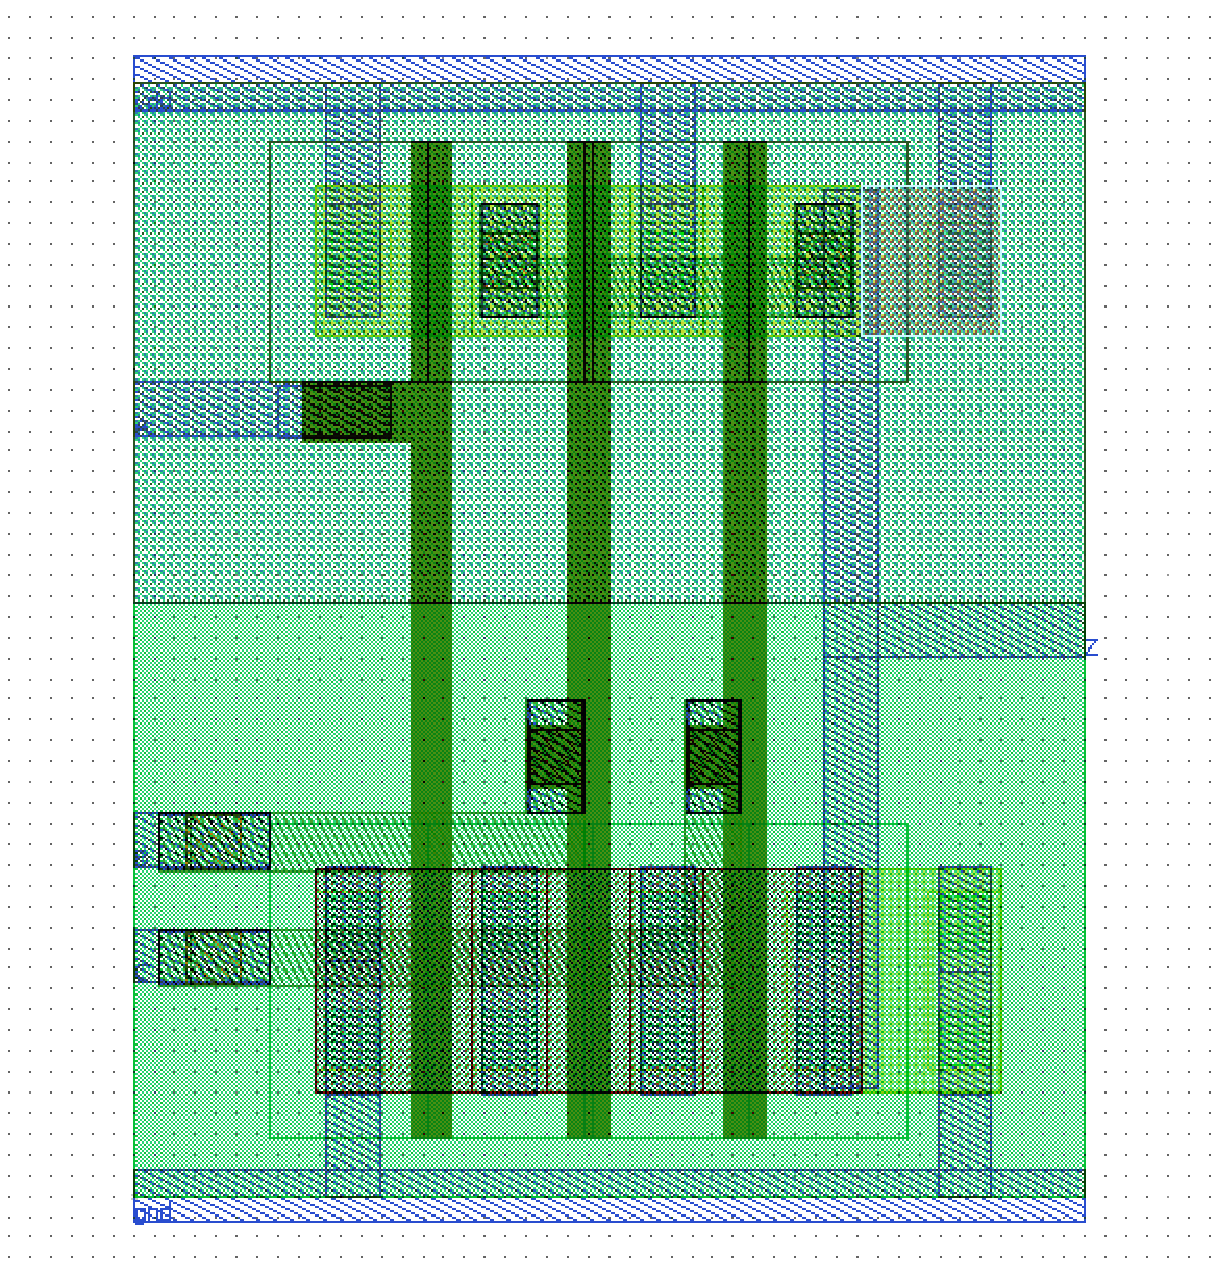
\includegraphics[width=10cm]{./figs/nand3.pdf}
\caption{An example of Parameterized NAND3(nand\_3)}
\label{fig:nand3}
\end{figure}

The \verb|nand_3| parameters are explained in Table~\ref{table:nand3_params}.
\begin{table}[h!] 
  \begin{center}
    \begin{tabular}{| l | c |}
    \hline
    Parameter & Explanation \\ \hline
    \verb|nmos_width| & The logic size of the transistor of the nmos in the nand3 \\ \hline
    \verb|height| = tech.cell\_6t[height] & physical dimension of cell height. \\ 
    \hline
    \end{tabular}
  \end{center}
  \caption{Parameter Explanation of nand3}
  \label{table:nand3_params}
\end{table}


\subsection{Parameterized NOR2}
\label{sec:nor2}

The parameterized nor2 (\verb|nor_2|) class generated a 2-input nor gate
of a specified size/strength and height.  The \verb|nor_2| is
constructed as follows:
\begin{verbatim}
def __init__(self, name, nmos_width, height=tech.cell_6t[height])
\end{verbatim}
The NMOS size is an input parameter, and the PMOS size
will be equal to $2$ NMOS size to have the equal rising and falling for output.
The following code instatiates the \verb|nor_2| instance seen in Figure~\ref{fig:nor2}.
\begin{verbatim}
a=nor_2.nor_2(name="nor2", nmos_width=2*tech.drc["minwidth_tx"], 
height=tech.cell_6t["height"])
\end{verbatim}


\begin{figure}[h!]
\centering
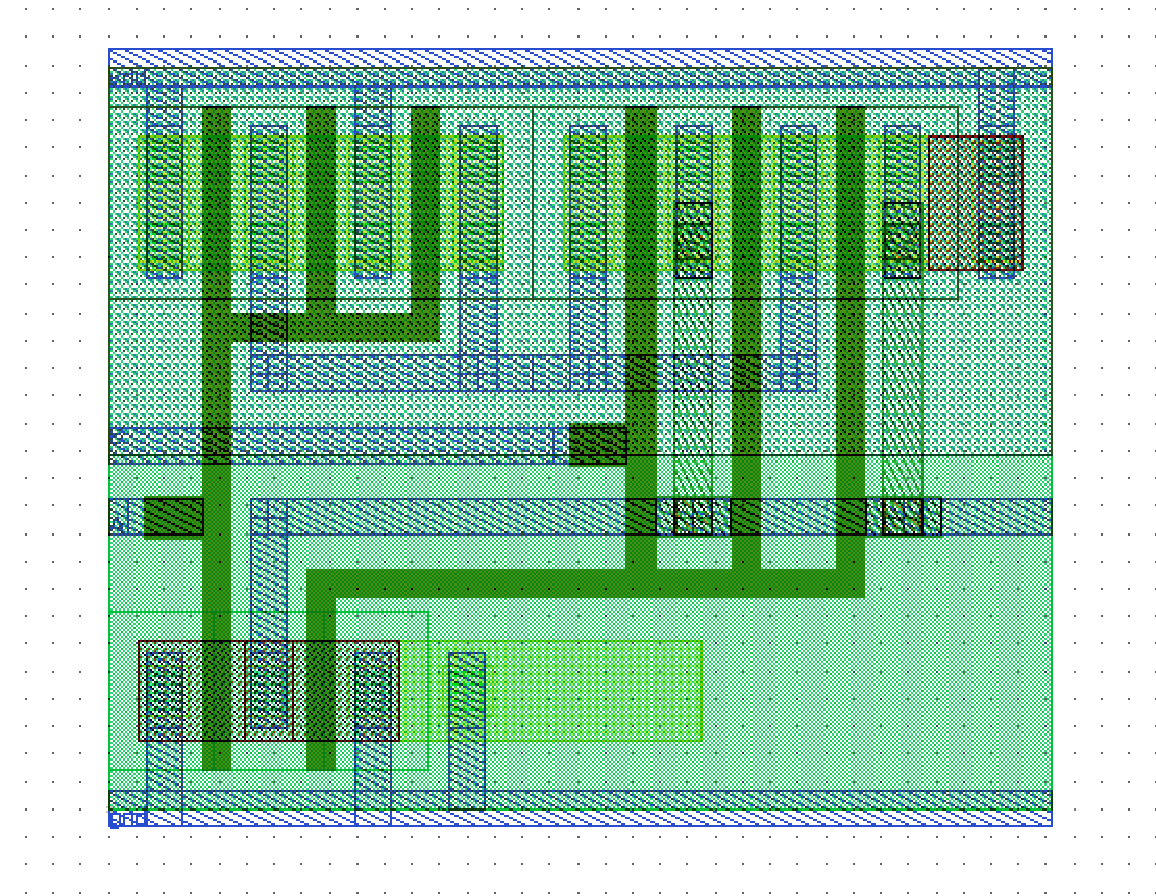
\includegraphics[width=10cm]{./figs/nor2.pdf}
\caption{An example of Parameterized NOR2(nor\_2)}
\label{fig:nor2}
\end{figure}

The \verb|nor_2| parameters are explained in Table~\ref{table:nor2_params}.
\begin{table}[h!] 
  \begin{center}
    \begin{tabular}{| l | c |}
    \hline
    Parameter & Explanation \\ \hline
    \verb|nmos_width| & The logic size of the transistor of the nmos in the nor2 \\ \hline
    \verb|height| = tech.cell\_6t[height] & physical dimension of cell height. \\ 
    \hline
    \end{tabular}
  \end{center}
  \caption{Parameter Explanation of nor2}
  \label{table:nor2_params}
\end{table}



\subsection{Path and Wire}
\label{sec:path and wire}
OpenRam provides two routing classes in custom layout design.
Both Path and wire class will take a set of coordinates connect those points 
with rectilinear metal connection.

The difference is that path only use the same layers for both vertical and 
horizontal connection while wire will use two different adjacent metal layers.
The this example will construct a metal1 layer path
\begin{verbatim}
layer_stack = ("metal1")
position_list = [(0,0), (0,3), (1,3), (1,1), (4,3)]
w=path.path(layer_stack,position_list) 
\end{verbatim}
and This exmaple will construct a wire using metal1 for vertical connection and metal2 for 
horizontal connection:
\begin{verbatim}
layer_stack = ("metal1","via1","metal2")
position_list = [(0,0), (0,3), (1,3), (1,1), (4,3)]
w=wire.wire(layer_stack,position_list)
\end{verbatim}



